\documentclass{article}

\usepackage{amsmath}
\usepackage{amssymb}
\usepackage{fancybox}
\usepackage{tikz}
\usepackage{comment}


\usepackage{cite}

\usepackage{listings}
\usepackage{color}
\usepackage{hyperref}

\definecolor{mygreen}{rgb}{0,0.6,0}
\definecolor{mygray}{rgb}{0.5,0.5,0.5}
\definecolor{mymauve}{rgb}{0.58,0,0.82}

\lstset{ %
  backgroundcolor=\color{white},   % choose the background color; you must add \usepackage{color} or \usepackage{xcolor}
  basicstyle=\footnotesize,        % the size of the fonts that are used for the code
  breakatwhitespace=false,         % sets if automatic breaks should only happen at whitespace
  breaklines=true,                 % sets automatic line breaking
  captionpos=b,                    % sets the caption-position to bottom
  commentstyle=\color{mygreen},    % comment style
  % deletekeywords={...},            % if you want to delete keywords from the given language
  escapeinside={\%*}{*)},          % if you want to add LaTeX within your code
  extendedchars=true,              % lets you use non-ASCII characters; for 8-bits encodings only, does not work with UTF-8
  frame=single,                    % adds a frame around the code
  keepspaces=true,                 % keeps spaces in text, useful for keeping indentation of code (possibly needs columns=flexible)
  keywordstyle=\color{blue},       % keyword style
  language=Octave,                 % the language of the code
  % otherkeywords={*,...},           % if you want to add more keywords to the set
  numbers=left,                    % where to put the line-numbers; possible values are (none, left, right)
  numbersep=5pt,                   % how far the line-numbers are from the code
  numberstyle=\tiny\color{mygray}, % the style that is used for the line-numbers
  rulecolor=\color{black},         % if not set, the frame-color may be changed on line-breaks within not-black text (e.g. comments (green here))
  showspaces=false,                % show spaces everywhere adding particular underscores; it overrides 'showstringspaces'
  showstringspaces=false,          % underline spaces within strings only
  showtabs=false,                  % show tabs within strings adding particular underscores
  stepnumber=2,                    % the step between two line-numbers. If it's 1, each line will be numbered
  stringstyle=\color{mymauve},     % string literal style
  tabsize=2,                   % sets default   tabsize to 2 spaces
  title=\lstname                   % show the filename of files included with \lstinputlisting; also try caption instead of title
}

% \language=[Objective]{Caml}




\title{Example binary search trees}
\date{\today}
\author{David M. Doolin}


\begin{document}

\maketitle

\abstract{A few notes on binary search trees and their implementations
in various programming languages.}



\section{Introduction}


\section{Literature review}

Skiena~\cite[pp. 77, 370, 375, 589]{skiena} has a few notes.

Aho and Ullman~\cite[pp. 210]{rosen} define height and depth for nodes in a binary tree.

\begin{quote}
The height of a node n is the length of a longest path from n to
a leaf. The height of the tree is the height of the root. The depth or level of
a node n is the length of the path from the root to n.
\end{quote}

Cormen et al.~\cite{cormen:th:1990} remains a classic reference.

Rosen~\cite[pp. 757-760]{rosen} discusses three uses for binary search trees:

\begin{enumerate}
\item storing items from a list such that they can be easily found;
\item finding an object in a collection of similar objects;
\item efficiently encoding characters in a bit string.
\end{enumerate}

\subsection{Collisions or duplicate values}

Inserting duplicate keys adds complexity.

\begin{itemize}
\item The duplicate key can be added to the tree, either silently or with a warning.
\item The duplicate key is not added to the tree, either silently or with a warning.

\item In Ruby, does replacing a node in a tree leak memory, or will the deleted node
get garbage collected? How about Python?

\item How to delete in c/c++ such that memory isn't leaked? This should be easier,
call delete after the node is orphaned.
\end{itemize}

\section{References}

\bibliography{references}{}
\bibliographystyle{plain}

\appendix


\section{The Generator trees}

\subsection{Tree 1}

%% Note the scale=0.5, which does exactly what is needed, reducing the
%% linear scale for all parts of the diagram, resulting in 1/4 the area.
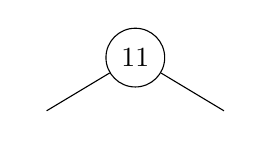
\begin{tikzpicture}[scale=0.5,level/.style={sibling distance=50mm/#1}]
  \node [circle,draw] (z) {$11$}
    child {
      node (a) {}
    }
    child {
      node (ca) {}
    };
\end{tikzpicture}


\subsection{Tree 2}

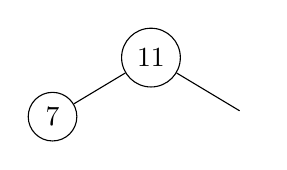
\begin{tikzpicture}[scale=0.5,level/.style={sibling distance=50mm/#1}]
  \node [circle,draw] (z) {$11$}
    child {
      node [circle,draw] (a) {$7$}
    }
    child {
      node (ca) {}
    };
\end{tikzpicture}

\subsection{Tree 3}

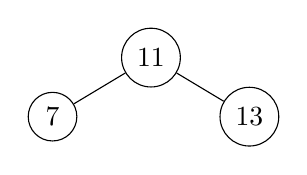
\begin{tikzpicture}[scale=0.5,level/.style={sibling distance=50mm/#1}]
  \node [circle,draw] (z) {$11$}
    child {node [circle,draw] (a) {$7$}}
    child {node [circle,draw] (ca) {$13$}};
\end{tikzpicture}

\subsection{Tree 4}

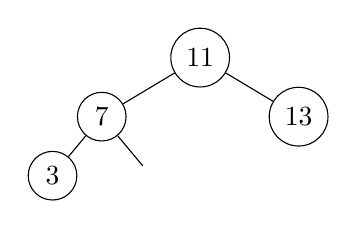
\begin{tikzpicture}[scale=0.5,level/.style={sibling distance=50mm/#1}]
  \node [circle,draw] (z){$11$}
    child {node [circle,draw] (a) {$7$}
      child {node [circle,draw] (j) {$3$}}
      child {node (ca) {}}
    }
    child {node [circle,draw] (ca) {$13$}};
\end{tikzpicture}

\subsection{Tree 5}

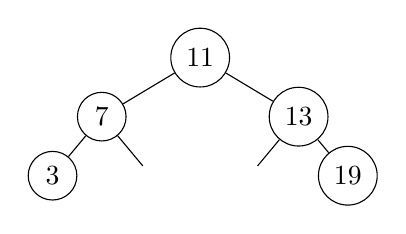
\begin{tikzpicture}[scale=0.5,level/.style={sibling distance=50mm/#1}]
  \node [circle,draw] (z){$11$}
    child {
      node [circle,draw] (a) {$7$}
        child {node [circle,draw] (j) {$3$}}
        child {node (ca) {}}
      }
    child {
      node [circle,draw] (ca) {$13$}
        child {node (a) {}}
        child {node [circle,draw] (j) {$19$}}
    };
\end{tikzpicture}


\subsection{Tree 6}

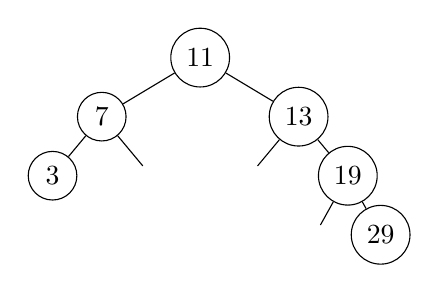
\begin{tikzpicture}[scale=0.5,level/.style={sibling distance=50mm/#1}]
  \node [circle,draw] (z){$11$}
    child {
      node [circle,draw] (a) {$7$}
        child {node [circle,draw] (j) {$3$}}
        child {node (ca) {}}
      }
    child {
      node [circle,draw] (ca) {$13$}
        child {node (a) {}}
        child {
          node [circle,draw] (j) {$19$}
          child {node (d) {}}
          child {
            node [circle,draw] (b) {$29$}
          }
        }
    };
\end{tikzpicture}

\subsection{Tree 7}

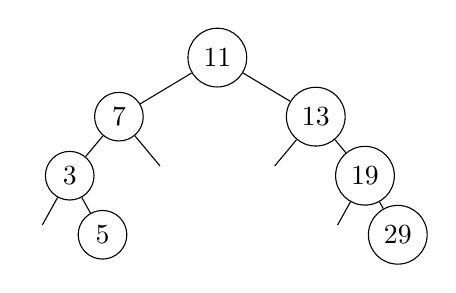
\begin{tikzpicture}[scale=0.5,level/.style={sibling distance=50mm/#1}]
  \node [circle,draw] (z){$11$}
    child {
      node [circle,draw] (a) {$7$}
        child {
          node [circle,draw] (j) {$3$}
            child {
              node (g) {}
            }
            child {
              node [circle,draw] (u) {$5$}
            }
        }
        child {
          node (ca) {}
        }
      }
    child {
      node [circle,draw] (ca) {$13$}
        child {node (a) {}}
        child {
          node [circle,draw] (j) {$19$}
          child {node (d) {}}
          child {
            node [circle,draw] (b) {$29$}
          }
        }
    };
\end{tikzpicture}


\subsection{Tree 8}

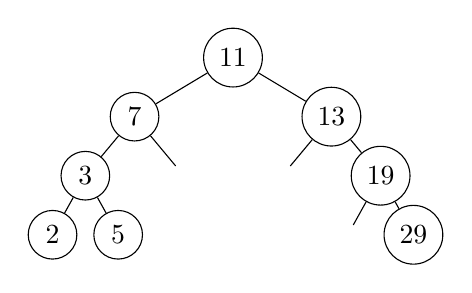
\begin{tikzpicture}[scale=0.5,level/.style={sibling distance=50mm/#1}]
  \node [circle,draw] (z){$11$}
    child {
      node [circle,draw] (a) {$7$}
        child {
          node [circle,draw] (j) {$3$}
            child {
              node [circle,draw] (g) {$2$}
            }
            child {
              node [circle,draw] (u) {$5$}
            }
        }
        child {
          node (ca) {}
        }
      }
    child {
      node [circle,draw] (ca) {$13$}
        child {node (a) {}}
        child {
          node [circle,draw] (j) {$19$}
          child {node (d) {}}
          child {
            node [circle,draw] (b) {$29$}
          }
        }
    }
;
\end{tikzpicture}


\subsection{Tree 9}

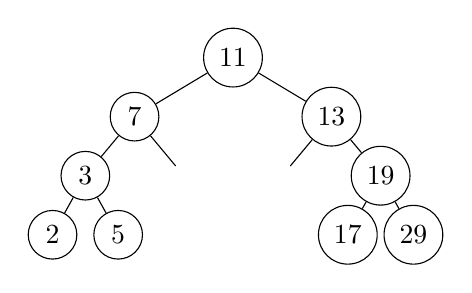
\begin{tikzpicture}[scale=0.5,level/.style={sibling distance=50mm/#1}]
  \node [circle,draw] (z){$11$}
    child {
      node [circle,draw] (a) {$7$}
        child {
          node [circle,draw] (j) {$3$}
            child {
              node [circle,draw] (g) {$2$}
            }
            child {
              node [circle,draw] (u) {$5$}
            }
        }
        child {
          node (ca) {}
        }
      }
    child {
      node [circle,draw] (ca) {$13$}
        child {node (a) {}}
        child {
          node [circle,draw] (j) {$19$}
          child {
            node [circle,draw] (d) {$17$}
          }
          child {
            node [circle,draw] (b) {$29$}
          }
        }
    }
;
\end{tikzpicture}

\subsection{Tree 10}

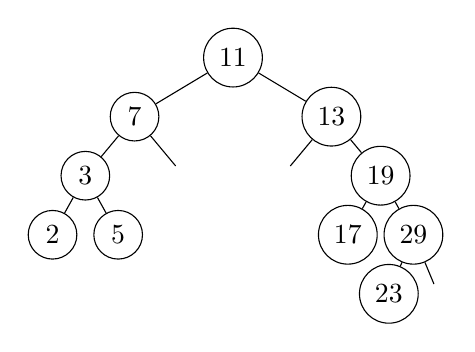
\begin{tikzpicture}[scale=0.5,level/.style={sibling distance=50mm/#1}]
  \node [circle,draw] (z){$11$}
    child {
      node [circle,draw] (a) {$7$}
        child {
          node [circle,draw] (j) {$3$}
            child {
              node [circle,draw] (g) {$2$}
            }
            child {
              node [circle,draw] (u) {$5$}
            }
        }
        child {
          node (ca) {}
        }
      }
    child {
      node [circle,draw] (ca) {$13$}
        child {node (a) {}}
        child {
          node [circle,draw] (j) {$19$}
            child {
              node [circle,draw] (d) {$17$}
            }
            child {
              node [circle,draw] (b) {$29$}
                child {
                  node [circle,draw] (e) {$23$}
                }
                child {
                  node (f) {}
                }
            }
        }
    }
;
\end{tikzpicture}



\section{The 5 $123$ trees}

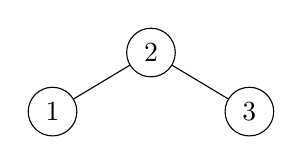
\begin{tikzpicture}[scale=0.5,level/.style={sibling distance=50mm/#1}]
  \node [circle,draw] (z){$2$}
    child {node [circle,draw] (a) {$1$}}
    child {node [circle,draw] (j) {$3$}
  };
\end{tikzpicture}

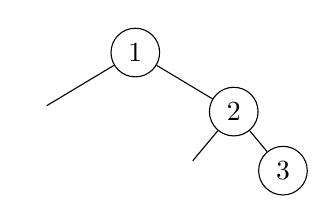
\begin{tikzpicture}[scale=0.5,level/.style={sibling distance=50mm/#1}]
  \node [circle,draw] (z){$1$}
  child {node (ca) {}}
  child {node [circle,draw] (a) {$2$}
    child {node (ca) {}}
    child {node [circle,draw] (j) {$3$}}
  };
\end{tikzpicture}

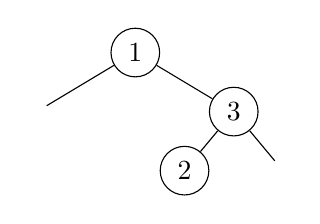
\begin{tikzpicture}[scale=0.5,level/.style={sibling distance=50mm/#1}]
  \node [circle,draw] (z){$1$}
  child {
    node (ca) {}
  }
  child {
    node [circle,draw] (a) {$3$}
      child {node [circle,draw] (j) {$2$}}
      child {node (ca) {}}
  };
\end{tikzpicture}

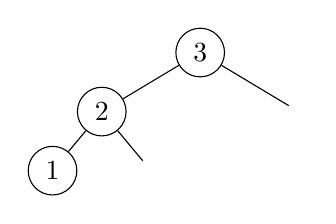
\begin{tikzpicture}[scale=0.5,level/.style={sibling distance=50mm/#1}]
  \node [circle,draw] (z){$3$}
  child {
    node [circle,draw] (a) {$2$}
      child {node [circle,draw] (j) {$1$}}
      child {node (ca) {}}
  }
  child {
    node (ca) {}
  };
\end{tikzpicture}


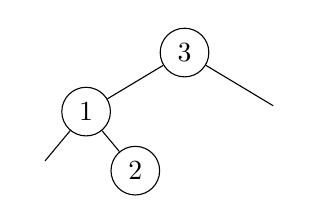
\begin{tikzpicture}[scale=0.5,level/.style={sibling distance=50mm/#1}]
  \node [circle,draw] (z){$3$}
  child {
    node [circle,draw] (a) {$1$}
      child {node (ca) {}}
      child {node [circle,draw] (j) {$2$}}
  }
  child {
    node (ca) {}
  };
\end{tikzpicture}



\vspace{.2in}
\hrule
\vspace{.2in}


A binary search tree using first 10 primes for keys:

%\ovalbox{%
  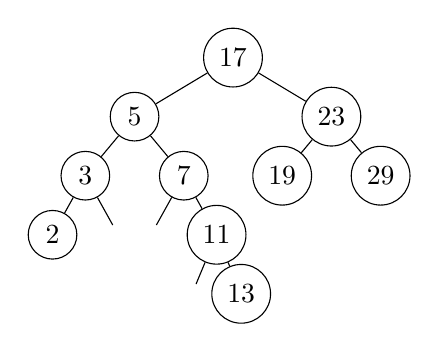
\begin{tikzpicture}[scale=0.5,level/.style={sibling distance=50mm/#1}]
  \node [circle,draw] (z){$17$}
    child {node [circle,draw] (a) {$5$}
      child {node [circle,draw] (b) {$3$}
        child {node [circle, draw] (c) {$2$}}
        child {node (ca) {}}
      }
      child {node [circle,draw] (g) {$7$}
        child {node (ga) {}}
        child {node [circle,draw] (gb) {$11$}
          child {node {}}
          child {node [circle,draw] (gc) {$13$}}
        }
      }
    }
    child {node [circle,draw] (j) {$23$}
      child {node [circle,draw] (k) {$19$}}
    child {node [circle,draw] (l) {$29$}}
  };
\end{tikzpicture}
%}



\section{Tikz}

% \href{http://www.texample.net/tikz/examples/merge-sort-recursion-tree/}{From texample.net}

\ovalbox{%
  \begin{tikzpicture}[level/.style={sibling distance=50mm/#1}]
  \node [circle,draw] (z){$17$}
    child {node [circle,draw] (a) {$5$}
      child {node [circle,draw] (b) {$3$}
        child {node [circle, draw] (c) {$2$}}
        child {node (ca) {}}
      }
      child {node [circle,draw] (g) {$7$}
        child {node (ga) {}}
        child {node [circle,draw] (gb) {$11$}
          child {node {}}
          child {node [circle,draw] (gc) {$13$}}
        }
      }
    }
    child {node [circle,draw] (j) {$23$}
      child {node [circle,draw] (k) {$19$}}
    child {node [circle,draw] (l) {$29$}}
  };
\end{tikzpicture}
}



\href{http://www.texample.net/tikz/examples/merge-sort-recursion-tree/}{From texample.net}

\ovalbox{%
%\begin{tikzpicture}[level/.style={sibling distance=60mm/#1}]
\begin{tikzpicture}[level/.style={sibling distance=40mm/#1}]
\node [circle,draw] (z){$n$}
  child {node [circle,draw] (a) {$\frac{n}{2}$}
    child {node [circle,draw] (b) {$\frac{n}{2^2}$}
      child {node {$\vdots$}
        child {node [circle,draw] (d) {$\frac{n}{2^k}$}}
        child {node [circle,draw] (e) {$\frac{n}{2^k}$}}
      }
      child {node {$\vdots$}}
    }
    child {node [circle,draw] (g) {$\frac{n}{2^2}$}
      child {node {$\vdots$}}
      child {node {$\vdots$}}
    }
  }
  child {node [circle,draw] (j) {$\frac{n}{2}$}
    child {node [circle,draw] (k) {$\frac{n}{2^2}$}
      child {node {$\vdots$}}
      child {node {$\vdots$}}
    }
  child {node [circle,draw] (l) {$\frac{n}{2^2}$}
    child {node {$\vdots$}}
    child {node (c){$\vdots$}
      child {node [circle,draw] (o) {$\frac{n}{2^k}$}}
      child {node [circle,draw] (p) {$\frac{n}{2^k}$}
        child [grow=right] {node (q) {$=$} edge from parent[draw=none]
          child [grow=right] {node (q) {$O_{k = \lg n}(n)$} edge from parent[draw=none]
            child [grow=up] {node (r) {$\vdots$} edge from parent[draw=none]
              child [grow=up] {node (s) {$O_2(n)$} edge from parent[draw=none]
                child [grow=up] {node (t) {$O_1(n)$} edge from parent[draw=none]
                  child [grow=up] {node (u) {$O_0(n)$} edge from parent[draw=none]}
                }
              }
            }
            child [grow=down] {node (v) {$O(n \cdot \lg n)$}edge from parent[draw=none]}
          }
        }
      }
    }
  }
};
\path (a) -- (j) node [midway] {+};
\path (b) -- (g) node [midway] {+};
\path (k) -- (l) node [midway] {+};
\path (k) -- (g) node [midway] {+};
\path (d) -- (e) node [midway] {+};
\path (o) -- (p) node [midway] {+};
\path (o) -- (e) node (x) [midway] {$\cdots$}
  child [grow=down] {
    node (y) {$O\left(\displaystyle\sum_{i = 0}^k 2^i \cdot \frac{n}{2^i}\right)$}
    edge from parent[draw=none]
  };
\path (q) -- (r) node [midway] {+};
\path (s) -- (r) node [midway] {+};
\path (s) -- (t) node [midway] {+};
\path (s) -- (l) node [midway] {=};
\path (t) -- (u) node [midway] {+};
\path (z) -- (u) node [midway] {=};
\path (j) -- (t) node [midway] {=};
\path (y) -- (x) node [midway] {$\Downarrow$};
\path (v) -- (y)
  node (w) [midway] {$O\left(\displaystyle\sum_{i = 0}^k n\right) = O(k \cdot n)$};
\path (q) -- (v) node [midway] {=};
\path (e) -- (x) node [midway] {+};
\path (o) -- (x) node [midway] {+};
\path (y) -- (w) node [midway] {$=$};
\path (v) -- (w) node [midway] {$\Leftrightarrow$};
\path (r) -- (c) node [midway] {$\cdots$};
\end{tikzpicture}}


\end{document}
